\section{Bresenham算法在三维空间中的应用与拓展}
\subsection{Bresenham算法简述\cite{计算机图形学基础}}
直线的绘制首先要考虑的是直线绘制的质量,有以下标准:
\begin{itemize}
    \item 直线要直,所选像素点应尽量靠近理想直线。
    \item 直线的端点要准确,保证绘制无定向性,即从$A$点到$B$点画一条直线同从$B$点到$A$点画一条直线应重合,且在绘制多条端点相连的直线时,不会因算法的累计错误造成断裂和不连接的情况。
    \item 相同设备下画线的速度应尽可能的快。
\end{itemize}
\subsubsection{Bresebham算法绘制二维直线\cite{计算机图形学基础}}
给定直线的两个端点$P_0(x_0,y_0)$和$P_1(x_1,y_1)$,可得到直线方程
\begin{align}
    F(x,y)=y-kx-b=0\\
    k=\frac{\Delta y}{\Delta x}=\frac{Y_1-Y_0}{X_1-X_0}
\end{align}
\par
这时直线将平面分为三个区域:对于直线上的点,$F(x,y)=0$;对于直线上方的点,$F(x,y)>0$;对于直线下方的点,$F(x,y)<0$,如图\ref{pic:直线将平面分为三个区域}所示。
\begin{figure}[H]
	\centering
	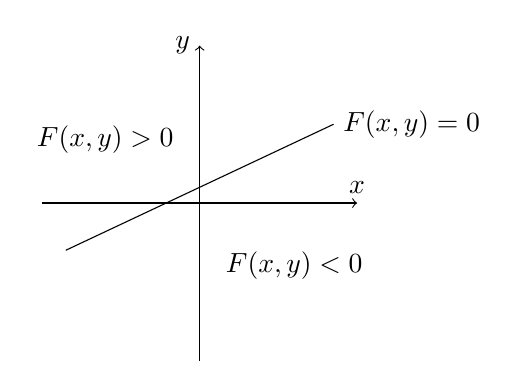
\begin{tikzpicture}[scale=1]
		\draw [->] (-2,0) -- (2,0) node[above]{$x$};
		\draw [->] (0,-2) -- (0,2) node[left]{$y$};
		\draw (-1.7,-.6) -- (1.7,1) node[right]{$F(x,y)=0$};
		\draw (-1.2,.5) node[above]{$F(x,y)>0$} (1.2,-.5) node[below]{$F(x,y)<0$};
	\end{tikzpicture}
	\caption{直线将平面分为三个区域}
	\label{pic:直线将平面分为三个区域}
\end{figure}
\par
由$Bresenham$提出的直线生成算法的基本原理是,每次在最大位移方向上走一步,而另一个方向是走步还是不走步取决于误差项的判别,如图\ref{pic:Brensemham算法生成直线的原理}所示。
\begin{figure}[H]
	\centering
	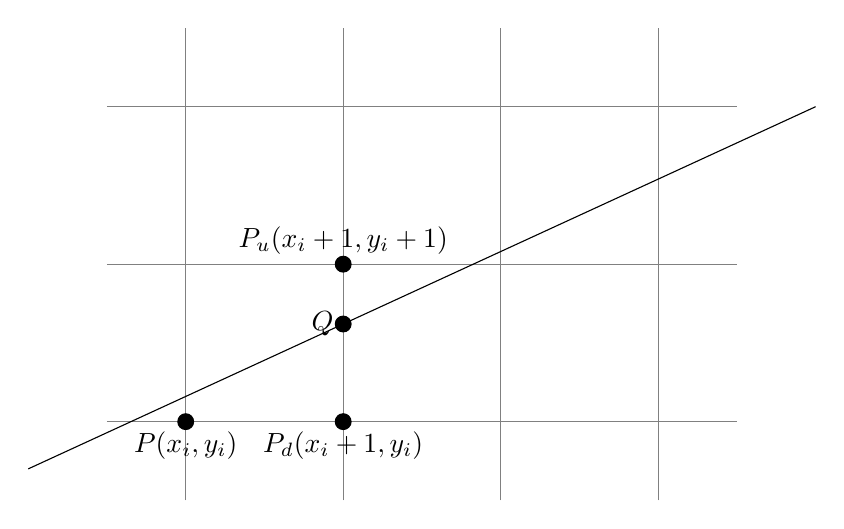
\begin{tikzpicture}[scale=2]
		\draw [help lines] (-.5,-.5) grid (3.5,2.5);
		\draw (-1,-.3) -- (4,2);
		\draw [fill]
		(0,0) circle [radius=0.05] node [below] {$P(x_i,y_i)$}
		(1,0) circle [radius=0.05] node [below] {$P_d(x_i+1,y_i)$}
		(1,1) circle [radius=0.05] node [above] {$P_u(x_i+1,y_i+1)$}
		(1,.62) circle [radius=0.05] node [left] {$Q$};
	\end{tikzpicture}
	\caption{Brensemham算法生成直线的原理}
	\label{pic:Brensemham算法生成直线的原理}
\end{figure}
\par
假定$0\leq k \leq 1$,由于$x$是最大位移方向,因此每次在$x$方向上加$1$,$y$方向上或加$1$,或加$0$。
假设当前点是$P(x_i,y_i)$,则下一个点在$P_u(x_i+1,y_i+1)$与$P_d(x_i+1,y_i)$中选一。
设$Q$是理想直线与垂直直线$x=x_i+1$的交点;
显然,若$|\overrightarrow{P_d Q}|>0.5$,则$P_u(x_i+1,y_i+1)$离直线近,否则$P_d(x_i+1,y_i)$离直线近。
\par
如前所述,直线方程为$F(x,y)=|y-kx-b|$。欲判断$|\overrightarrow{P_d Q}|$,只要把$P_d$代入$F(x,y)$,并判断它与$0.5$的大小即可。
\par
构造判式如下:
\begin{equation}
d_i=F(x_i+1,y_i)=y_i-kx_i-k-b
\label{math:bresenham二维直线判别式}
\end{equation}
\par
当$d_i \leq 0.5$时,应取$P_u$。当$d_i > 0.5$时,则应取正右方的$P_d$,即
\[
\left\{
\begin{array}{ll}
	x_{i+1}&=x_i+1\\
	y_{i+1}&=\left\{
	\begin{array}{ll}
	y_i+1 & (d_i>0.5) \\
	y_i & (d_i \leq 0.5)
	\end{array}
	\right.
\end{array}	
\right.
\]
\par
其中的关键在于误差项$d_i$,它的初始值为$0$,每走一步有$d_{i+1}=d_i+k(k=\frac{\Delta y}{\Delta x},\textbf{为直线斜率})$。一旦$y$方向上走了一步,就把它减去$1$(此时可能出现负误差,这表明交点在所取网格点之下)。为计算方便,令$e_i=d_i-0.5$。则当$e_i>0$时,下一像素的$y$坐标增加$1$;否则,下一像素的$y$坐标不增,即有
\[
\left\{
\begin{array}{ll}
	x_{i+1}&=x_i+1\\
	y_{i+1}&=\left\{
	\begin{array}{ll}
		y_i+1 & (e_i>0) \\
		y_i & (e_i \leq 0)
	\end{array}
	\right.
\end{array}	
\right.
\]
\par
此时,$e_i$的初值为$-0.5$,每走一步有$e_{i+1}=e_i+k$。当$e_i>0$时(相当于$y$方向上走一步时),将$e_i$减$1$。
\begin{figure}[H]
	\centering
	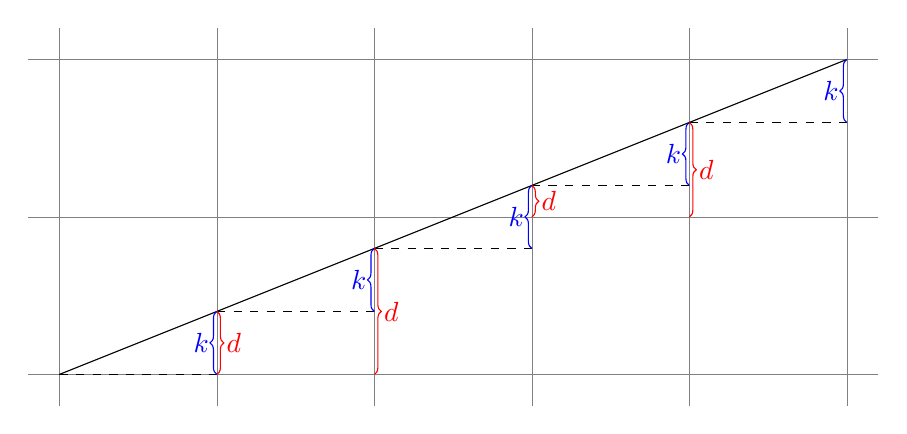
\begin{tikzpicture}[scale=2]
		\draw [help lines] (-.2,-.2) grid (5.2,2.2);
		\draw (0,0) -- (5,2);
		\foreach \x in {0,1,2,3,4}
		{
			\draw [dashed] (\x,\x*2/5) -- (\x+1,\x*2/5);
			\draw [decorate,decoration={brace},blue] (\x+1,\x*2/5) -- (\x+1,\x*2/5+2/5) node [xshift=-0.2cm,yshift=-.4cm] {$k$};
		};
		\draw [decorate,decoration={brace},red] (1,.4) -- (1,0);
		\draw [decorate,decoration={brace},red] (2,.8) -- (2,0);
		\draw [decorate,decoration={brace},red] (3,1.2) -- (3,1);
		\draw [decorate,decoration={brace},red] (4,1.6) -- (4,1);
		\draw [red,right]
		(1,.2) node {$d$}
		(2,.4) node {$d$}
		(3,1.1) node {$d$}
		(4,1.3) node {$d$};
	\end{tikzpicture}
	\caption{Brensemham算法绘制直线的原理}
	\label{pic:Brensemham算法绘制直线的原理}
\end{figure}
\par
\subsubsection{Bresebham算法绘制二维椭圆}
\subsection{Bresenham算法绘制三维直线}
\subsection{Bresenham算法绘制三维椭圆}
\subsection{Bresenham算法绘制三维椭球}
